\chapter{Конструкторская часть}

В этом разделе представлена схема алгоритма шифровальной машины <<Энигма>>.

\section{Разработка алгоритмов}

На рисунках \ref{fig:des-ecb}--\ref{fig:des-f} представлены схемы алгоритмов DES, раунда DES, функции Фейстеля, а также режимы работы ECB при зашифровке и расшифровке.

\begin{figure}[ht!]
	\centering
	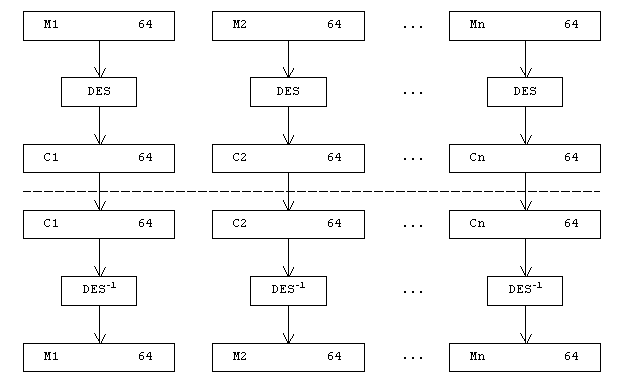
\includegraphics[width=0.9\linewidth]{img/des-ecb.png}
	\caption{Схема алгоритма DES в режиме ECB}
	\label{fig:des-ecb}
\end{figure}

\begin{figure}[ht!]
	\centering
	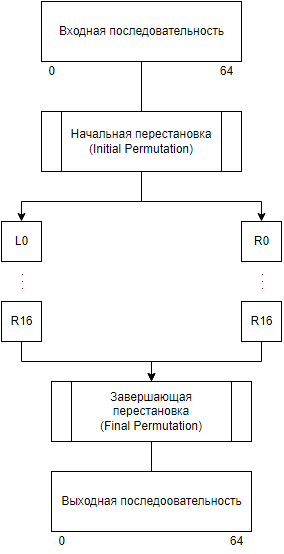
\includegraphics[width=0.4\linewidth]{img/des-al.png}
	\caption{Схема алгоритма DES}
	\label{fig:des-al}
\end{figure}

\begin{figure}[ht!]
	\centering
	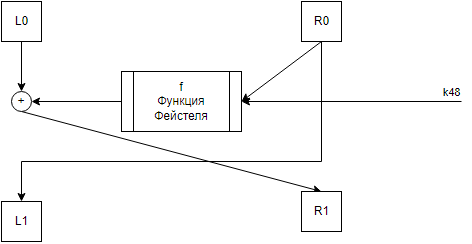
\includegraphics[width=0.6\linewidth]{img/round.png}
	\caption{Схема алгоритма раунда DES}
	\label{fig:des-round}
\end{figure}

\clearpage

\begin{figure}[ht!]
	\centering
	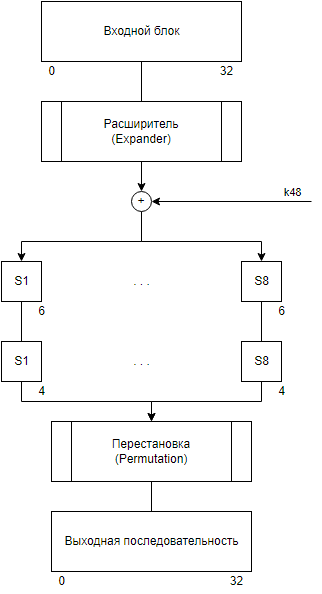
\includegraphics[width=0.5\linewidth]{img/function.png}
	\caption{Схема алгоритма функции Фейстеля}
	\label{fig:des-f}
\end{figure}

